
\chapter{Implementierungen}\label{s.Implementierungen}

\section{Strategie bei der Vorgehensweise}\label{Strategie bei der Vorgehensweise}
Zunächst wird eine Implementierung gewählt, die die besten Chancen hat, alle funktionalen und nicht funktionalen Anforderungen zu erfüllen. Dies ist eine Lösung in Javascript mit dem node.js-Framework und dem socket.io-Websocket (Abschnitt \ref{socket.io-Server} und \ref{socket.io-Client}). Node.js-Serveranwendungen werden schon länger mit guten Ergebnissen in Netzwerken eingesetzt, besonders für Realtime-Anwendungen mit vielen gleichzeitig verbunden Clients. Das socket.io-Paket wird genutzt, weil durch die Kapselung der verschiedenen Transportmechanismen die Bedienung einer maximalen Anzahl verschiedener Browser, auch in älteren Versionen möglich ist, ohne den Implementierungsaufwand unverhältmismäßig zu erhöhen. Die Implementierung dieser Lösung steht im Zeitplan ganz vorne, um der Anforderung von Unternehmensseite nach einer zeitnahen Umsetzung und Auslieferung zu entsprechen.
In einem zweiten Schritt wird eine vergleichbare Implementierung in Google Dart ausgeführt. Die Entwicklung von Dart befindet sich noch in der Beta-Phase. Der zweite Beta-Release fand im Dezember 2012 statt. Ein dritter Beta-Release ist angekündigt. Ein zeitnaher ausschließlicher Einsatz von Dart im Produktivsystem wird also in absehbarer Zeit nicht möglich sein, weshalb diese Lösung als Investition in die Zukunft anzusehen ist. 
Der Vergleich beider Implementierungen (Javascript vs. Dart) ist deshalb nicht weniger interessant.   
\section{Notwendige Strategie-Korrekturen}\label{Strategie-Korrektur}
Der ursprüngliche Plan, sowohl einen Server als auch einen Client in Dart zu schreiben, musste korrigiert werden, weil mit dem Dart-Websocket-Server einige der grundlegenden Anforderungen nicht umzusetzen waren. Zum einen unterstützt Dart keine JSON-over-TCP -Kommunikation, wie sie für die Abfrage des JSON-Datenstroms vom Rohdatenserver erforderlich ist. Und zum anderen gab es noch keinen Redis-Client für Dart. Der publish/subscribe Mechanismus der Redis-Datenbank wird für die Verteilung der Positionsupdates benötigt.
Deshalb wird nur die Clientanwendung in Dart implementiert (in Abschnitt \ref{HTML5-Client in Dart}). Dadurch ergibt sich ein weiteres Problem: Dart unterstützt Websockets nach der HTML5-Websocket-API-Spezifikation clientseitig mit dem Paket dart:html. Der socket.io-Websocket-Server entspricht nicht der HTML5-Websocket-API-Spezifikation und benötigt deshalb auf Clientseite zusätzliche Bibliotheken. Diese socket.io-client-Bibliotheken stehen in Dart nicht zur Verfügung. 
Also wird außer dem socket.io-Server ein zweiter Server implementiert, der eine Websocket-Verbindung nach der HTML5-Websocket-API-Spezifikation aufbaut (in Abschnitt \ref{HTML5-Server}). Die Umsetzung in node.js mit dem websocket-Modul  \footnote{https://github.com/Worlize/WebSocket-Node/wiki/Documentation} ist recht einfach möglich.
\section{Das Problem der Vergleichbarkeit}\label{Vergleichbarkeit}
An dieser Stelle stellt sich die Frage, ob beide Serverlösungen vergleichbare Ergebnisse liefern. Denn Unterschiede zwischen den node.js-Servern (socket.io vs. HTML5) würden in das Ergebnis des Vergleichs zwischen den Clients (Dart vs Javascript) einfliessen. Deshalb wird für den HTML5-kompatiblen Websocket-Server noch ein Javascript-Client geschrieben, der dann direkt vergleichbar ist mit dem in Dart geschriebenen Client.
Es bleibt noch zu beurteilen, inwieweit die Javascript-Implementierung durch den Verzicht auf das socket.io-Framework, das in der ersten Lösung verwendet wird, ausgebremst wird. Das geschieht über einen Performance-Vergleich in Abschnitt \ref {socket.io- vs html5-Server}.
Es werden also zwei Vergleiche durchgeführt: 
\begin{itemize}
\item In Javascript wird der socket.io-Websocket gegen den HTML5-Websocket getestet.
\item Unter Verwendung des HTML5-Websockets wird der Javascript-Client gegen den Dart-Client getestet
\end{itemize}
Tabelle\ref{tab:uebersicht} zeigt eine Übersicht über die Implementierungen.
Auf diese Weise wird die präferierte Lösung in node.js mit socket.io nicht unmittelbar sondern mittelbar über die Javascript-Lösung mit HTML5-Websocket gegen die Implementierung mit einem Google Dart Client getestet.
\renewcommand{\arraystretch}{2}

\begin{table}[!hbt]\vspace{1ex}\centering
\begin{tabular}{| l| m{3.5cm}||c|c|}\cline{3-4}

\multicolumn{2}{c||}{}&\multicolumn{2}{c|}{HTTP-Client}\\\cline{3-4}
\multicolumn{2}{c||}{}& Javascript& Google Dart\\\hline\hline
\multirow{2}*{\rotatebox{90}{HTTP-Server}}& socket.io-Websocket-Server  (\ref{socket.io-Server}) &  socket.io-Client  (\ref{socket.io-Client})& 
\includegraphics[width=0.2in]{images/x_red.jpeg}\\\cline{2-4}
&HTML5-Websocket-Server (\ref{HTML5-Server}) & HTML5-Client (\ref{HTML5-Client in Javascript}) & HTML5-Client  (\ref{HTML5-Client in Dart})\\\hline
\multicolumn{4}{c}{}\\
\end{tabular}
\caption[Übersicht über Server-und Clientimplementierungen in dieser Arbeit]
{Übersicht über Server-und Clientimplementierungen in dieser Arbeit\\}
\vspace{2ex}
\label{tab:uebersicht}
\end{table}
\newpage

\section{Beschreibung der ausgeführten Implementierungen}
In der ersten Implementierung werden Lösungen entwickelt für die in den Anforderungen beschriebenen Aufgaben. In allen weiteren Implementierungen werden diese Lösungen möglichst übernommen und andernfalls eine Alternative entwickelt.

\subsection{socket.io-Server}\label{socket.io-Server}
Die zu entwickelnde Serveranwendung hat grundsätzlich zwei Aufgaben: 
\begin{enumerate}
\item Daten über eine JSON-over-TCP-Verbindung vom Rohdatenserver abzurufen und
\item einen Websocket zu betreiben, der die Daten an Websocket-Clients weitergibt
\end{enumerate}
Weil Node.js singlethreaded ist (vgl. \ref{Node.js}), würde der Server beide Aufgaben in einem einzigen Prozess bearbeiten. Um das Potential an Parallelverabeitung eines Dualcore oder Multicore-Servers zu nutzen, ist des daher sinnvoll, mindestens zwei Prozesse zu generieren. Dazu wurde das node.js-Modul child\_process genutzt. Die Start-Datei master.js generiert damit zuerst einen Prozess, der den AIS-Daten-Client (aisData-client.js) abzweigt, um Daten vom Rohdaten-Server abzufragen und anschließend einen worker-Prozess (worker.js), um einen Websocket -Server für Client-Verbindungen zur Verfügung zu stellen (siehe Listing \ref{master.js}).
\begin{lstlisting}[caption=Generierung von Kindprozessen in master.js, firstnumber=16, label=master.js]
/* AIS-Client - Process*/
  child.fork(path.join(__dirname, 'aisData-client.js'));

/*worker- Process*/
  child.fork(path.join(__dirname, 'worker.js'));
\end{lstlisting}
Bei der Weitergabe der Daten durch den worker-Prozess sind zwei Fälle zu unterscheiden:
\begin{itemize}
\item ein Client verbindet sich neu oder ändert den Kartenausschnitt. In diesem Fall (Vessel-in-Bounds Request) sind die Schiffs-und Positionsdaten aller im Bereich (Bounds) befindlichen Schiffe an den Client zu senden (Kapitel \ref{Vessels-in-Bounds-Request}).
\item ein Schiff sendet ein Positions-Update, das an alle Clients verteilt werden muss, deren Kartenausschnitt die betreffende Schiffsposition enthält. Dieses Ereignis wird im Folgenden Vessel-Position-Update genannt (Kapitel \ref{Vessel-Position-Update}).
\end{itemize}
\subsubsection{Vessels-in-Bounds-Request}\label{Vessels-in-Bounds-Request}
Der Vessels-in-Bounds-Request macht eine Zwischenspeicherung der Daten unumgänglich. Wegen der großen Anzahl gleichzeitig empfangener Schiffe (weltweit ca. 60.000) und der Notwendigkeit, einen geographischen Index zu verwenden, wird einer persistenten gegenüber einer transienten Speicherung der Vorzug gegeben. 
\\Für die Persistierung wird hier MongoDB verwendet, weil MongoDB als NoSQL-Datenbank mit geringem Overhead schnelle Antwortzeiten und außerdem einen geographischen Index bietet. Der Serverprozess in aisData-client.js schreibt die Daten (siehe listing \ref{write in Mongo}) in eine MongoDB-Collection namens ‘vesselsCollection’. Die MMSI eines Schiffes ist eindeutig und wird als unique key verwendet (siehe Abschnitt \ref{Statische Schiffsdaten}). Über die Option upsert:true wird der Mongo Datenbank mitgeteilt, dass entweder ein insert-Befehl oder, falls die mmsi bereits in der MongoDB-Collection vorhanden ist, ein update-Befehl auf das entsprechende set auszuführen ist. 
\begin{lstlisting}[caption=Schreiben in die Datenbank in aisData-client.js, label=write in Mongo]
vesselsCollection.update(
  { mmsi: obj.mmsi },
  { $set: obj },
  { safe: false, upsert: true }
  );
\end{lstlisting}
In Listing \ref{2d-Index} ist zu sehen, wie über das Schlüsselwort “2d” der MongoDB-Geo-Index auf das Feld ‘pos’ mit den Koordinaten des Schiffes gesetzt wird. Damit ist garantiert, dass nicht jede Anfrage des Servers an die Datenbank sämtliche Datensätze durchlaufen muss, um die Schiffe in einem bestimmten geographischen Ausschnitt zu finden. Aufbau und Unterhalt des Geo-Indexes findet im aisData-client-Prozess statt, der schreibend auf die Datenbank zugreift.
\begin{lstlisting}[caption=Aufbau des Geo-Indexes in aisData-client.js, label= 2d-Index]
  vesselsCollection.ensureIndex({ pos: "2d", sog: 1, time_received: 1 }, function(err, result) {... });
  \end{lstlisting}
Dabei handelt es sich um einen zusammengesetzten Index, weil neben der Geo-Position auch die Geschwindigkeit und der Zeitpunkt des Empfangs der Nachricht Filterkriterien sind, wenn der zweite Prozess (worker.js) lesend auf die Datenbank zugreift. In Listing \ref{lst:query Mongo} ist zu sehen, wie der Prozess worker.js mit den vom Client in einem Vessels-in-Bounds-Request übermittelten Geo-Daten die MongoDb anfragt.
  \begin{lstlisting} [caption=Vessel-in-Bounds-query in worker.js, label=lst:query Mongo]
  var vesselCursor = vesselsCollection.find({
    pos: { $within: { $box: [ [bounds._southWest.lng,bounds._southWest.lat], [bounds._northEast.lng,bounds._northEast.lat] ] } },
    time_received: { $gt: (new Date() - 10 * 60 * 1000) },
    sog: { $exists:true },
    sog: { $gt: zoomSpeedArray[zoom]},
    sog: {$ne: 102.3}
  });
  vesselCursor.toArray(function(err, vesselData)  {
   client.sendUTF(JSON.stringify({ type: 'vesselsInBoundsEvent', vessels: vesselData}));
});
\end{lstlisting}

\subsubsection{Vessel-Position-Update}\label{Vessel-Position-Update}
Für die Kommunikation eines Vessel-Position-Updates (AIS-Nachrichtentyp 1-3) zwischen dem aisData-client.js-Prozess und dem worker.js-Prozess wird der publish/subscribe-Mechnismus einer Redis-Datenbank genutzt. Der aisData-client.js-Prozess publiziert jedes Positions-Update auf dem Kanal ‘vessel-Pos’ der Redis-Datenbank. Der worker.js-Prozess meldet sich als subscriber am Kanal ‘vessel-Pos’ der Redis-Datenbank an und wird so bei jedem Positions-Update benachrichtigt.
Um diese Nachricht an die betroffenen Websocket-Clients weiterzuleiten, ist eine serverseitige Verwaltung der Clients notwendig. Die Serveranwendung muss bei jeder Positionsmeldung wissen, welche Clients benachrichtigt werden müssen. Die Client-Verwaltung ist ein Feature des socket.io-Paketes. Für jeden Client wird bei der Registrierung zusätzlich das Zoomlevel der Karte und die Koordinaten gespeichert.
\begin{lstlisting}[caption= Speichern der übermittelten Client-Daten in worker.js, label=Speichern der übermittelten Client-Daten in worker.js]
io.sockets.on('connection', function(client) {
      log(' Connection from client accepted.');
      client.on('register', function(bounds, zoom) {
      client.set('zoom', zoom);
      client.set('bounds', bounds, function() {
        getVesselsInBounds(client, bounds, zoom);
      });
    });
    client.on('unregister', function() {
      client.del('bounds');
      client.del('zoom');
    });
  });
  \end{lstlisting}
  Bei jedem Vessel-Position-Update, das der worker.js-Prozess empfängt, geht er die Liste der Clients durch und benachrichtigt diejenigen, in deren Bereich das Positions-Update fällt.
\begin{lstlisting}[caption= Weiterleitung von Positions-Updates an Websocket-Clients in worker.js, label= Weiterleitung von Positions-Updates an Websocket-Clients in worker.js]
 redisClient.on('message', function(channel, message) {
    if (channel == 'vesselPos')  {
      ...
      var json = JSON.parse(message);
      ...
      var clients = io.sockets.clients();
      var lon = json.pos[0];
      var lat = json.pos[1];
      var sog = json.sog/10;
      var cog = json.cog/10;
      clients.forEach(function(client) {
        client.get('bounds', function(err, bounds) {
          if (bounds != null && lon != null && lat != null) 
          {
            /* check, if Client-Connection is affected by Vessel-Position-Update */
            if (positionInBounds(lon, lat, bounds)) 
            {
              client.get('zoom', function(err, zoom) 
              {
                if(sog !=null && sog > (zoomSpeedArray[zoom]) && sog != 102.3)
                {
                  client.emit('vesselPosEvent', message);
                }
          ...
  });
\end{lstlisting}
%-------------------------------------------------------------------------------------------------------------------------------------------
\begin{figure}[H]
  \centering
  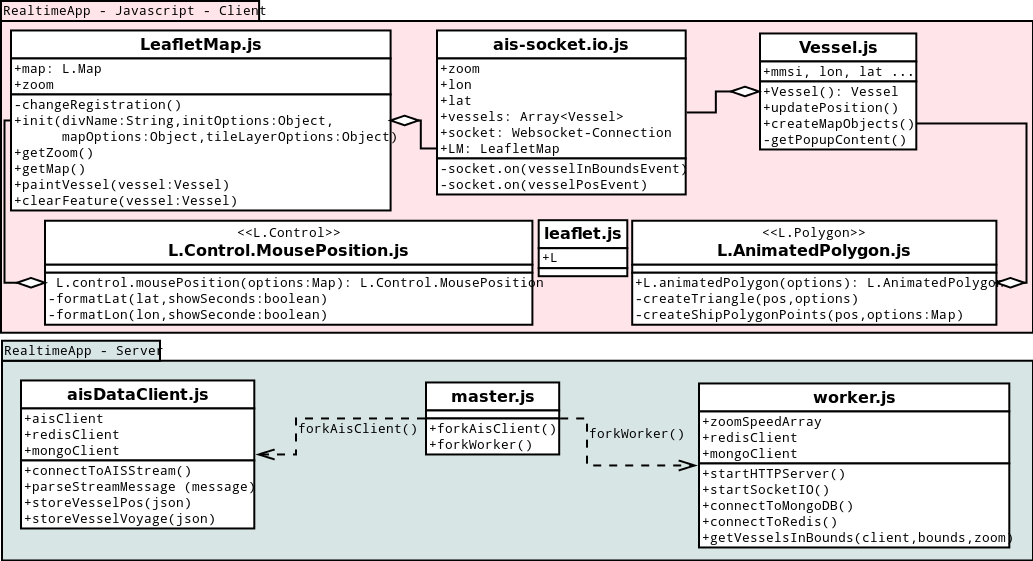
\includegraphics[width=6in]{images/Javascript-Dateien-undObjekte.png}
  \caption[Übersicht Javascript-Files]{Schematische Übersicht der implementierten Javascript-Dateien und -Objekte. In der Darstellung wird die Notation des UML-Klassendiagramms verwendet, was natürlich (Klassen existieren nicht in Javascript) nicht als solches gelesen werden kann. Weil aber die Anwendung obektorientiert konzipiert ist, war dieser Ansatz sowohl während der Entwicklung als auch bei der Beschreibung der Anwendung sehr nützlich. Die Attribute und Methoden sind nicht vollständig dargestellt, sondern so ausgewählt, dass Zusammenhänge und Abhängigkeiten erkennbar werden.
Dasselbe gilt für Abbildung  \ref{fig:Übersicht Dart-Files}, die den Dart-Client schematisch darstellt. }
  \label{fig:Übersicht Javascript-Files}
\end{figure}

\subsection{socket.io-Client}\label{socket.io-Client}
Der socket.io-Client hat folgende Aufgaben.
\begin{enumerate}
\item Es ist eine html-Seite zu erstellen, die die benötigten Source-Dateien lädt und eine HTML-Struktur aufbaut mit den DOM-Elementen für die Karte.
\item URL-Parameter sollen optional übergeben werden können.
\item Optionen sollen zentral an einer Stelle der Anwendung geändert werden können.
\item Eine Karte auf Basis des auf dem unternehmenseigenen Server gehosteten Kartenmaterials mit Navigations- und Infobereichen ist in den Kartenbereich zu rendern.
\item Zum Socket.io-Websocket-Server soll eine Verbindung aufgebaut werden, die
\begin{enumerate}
\item Vessel-In-Bounds- und Vessel-Position-Events empfängt und
\item bei Positionsänderungen auf der Karte eine register-Nachricht sendet
\end{enumerate}
\item Aus den empfangenen JSON-Daten sind geeignete Objekte zu erstellen und zu speichern.
\item Die Objekte sind als Features auf die Karte zu rendern
\item Objekte, die den Status ‘Moving’ haben, sind entsprechend ihrer Geschwindigkeit zu animieren.
\end{enumerate}
Punkt 1 geschieht in der Datei ais-socket.io.html, die zum Start der Anwendung vom Browser-Client aufgerufen wird. Dort werden die benötigten javascript- und css-Dateien eingebunden, inklusive der Jquery- und der Leaflet-Bibliothek. Nach dem Laden (on document.ready()) führt der Browser die Datei ais-socket.io.js aus. Falls Url-Parameter übergeben worden sind für initialen Zoomlevel und Kartenausschnitt (Punkt 2) werden sie nun mit der Funktion getParam(name) aufgegriffen, sonst wird ein Defaultwert für zoom und bounds benutzt. Wie unter Punkt 3 gefordert, kann dieser Defaultwert und alle weiteren Einstellungen (z.B. Server-IP, Server-Port, Map-Server-Url (Punkt 4)) in dieser Datei zentral angepasst werden.
Als Javascript-Bibliothek zur Darstellung der Schiffe auf der Karte wurde die Leaflet-Bibliothek (siehe Abschnitt \ref{Leaflet}) ausgewählt. Die Cockpit-Anwendung der Vesseltracker-GmbH nutzt die älteren OpenLayers-Bibliotheken, diese sind jedoch im Vergleich sehr viel sperriger in der Nutzung und werden inzwischen weniger aktiv von der Community weiterentwickelt und verbessert.
Mithilfe dieser Bibliothek wird die Karte als Javascript-Objekt in der Datei LeafletMap.js realisiert. Dazu wird das ‘Revealing Module Pattern’ genutzt, mit dem sich die API der Karte von ihrer internen Implementierung trennen lässt. Nur die in der return-Klausel zurückgegebenen Funktionen bilden die öffentliche Schnittstelle (Punkt 4). 

\begin{lstlisting}[caption= ‘Revealing Module Pattern’ in LeafletMap.js, label=LeafletMap.js]
var LMap = function(){
  var map, featureLayer, tileLayer, zoom, socket, boundsTimeout, boundsTimeoutTimer;
  function init(elementid, initOptions, mapOptions, tileLayerOptions) { ... }
  function changeRegistration() { ... } 
  function getMap(){ ... }
  function getZoom(){ ... }
  function addToMap(feature, animation, popupContent){ ... } 
  function removeFeatures(vessel){ ... }
  return {
    init: init,
    getMap: getMap,
    getZoom: getZoom,
    addToMap: addToMap,
    removeFeatures: removeFeatures }
}();
\end{lstlisting}
Nach dem Initialisieren der Karte wird die Websocket-Verbindung (Punkt 5) hergestellt (siehe listing \ref{ais-socket.io.js}). Für den Empfang der Nachrichten des Websocket-Servers (Punkt 5a, siehe auch Kapitel \ref{socket.io-Server}) genügen dazu zwei Listener: 
\begin{lstlisting}[caption=Client-Seite der socket.io-Websocket-Verbindung in ais-socket.io.js,  label=ais-socket.io.js]
 var socket = io.connect('http://'+WEBSOCKET_SERVER_LOCATION+':'+WEBSOCKET_SERVER_PORT);
socket.on('vesselsInBoundsEvent', function (data) {...}
socket.on('vesselPosEvent', function (data) {...}
\end{lstlisting}

Um eine Liste aller im Kartenbereich befindlichen Schiffe vom Server zu bekommen, muss der Client eine ‘register’-Nachricht mit den aktuellen Bounds an den Server senden (Punkt 5b, siehe dazu \ref{Speichern der übermittelten Client-Daten in worker.js}).
Dies geschieht einmal nach dem Intialisieren der Karte und soll anschließend durch den von der Leaflet-Map nach jeder Änderung des Kartenausschnitts getriggerten moveend-Event ausglöst werden, bzw. spätestens nach der als BOUNDS\_TIMEOUT übergebenen Zeitspanne. Weil dieser Event innerhalb des LeafletMap-Objektes auftritt, wird dem LeafletMap-Objekt bei der Initialisierung eine Referenz auf die Websocket-Connection übergeben. Diese Lösung ist unproblematisch, weil beim Verlust der socket-Verbindung ohnehin ein Reload der Seite stattfinden muss.\\
Um geeignete Objekte aus den Ais-Messages zu erstellen (Punkt 6), wird in der Datei Vessel.js eine Konstruktor-Funktion zur Verfügung gestellt, mit der Instanzen von Vessel-Objekten generiert werden können. Diese Instanzen werden in einem assoziativen Array, also einem Objekt, namens ‘vessels’ in ais-socket.io.js gespeichert. Beim Empfang eines Vessel-Position-Events kann mit vessels[mmsi] nach dem passenden vessel-Objekt zum Update gesucht werden.
Schließlich sind die Vessel-Objekte auf die Karte zu rendern (Punkt 7). Dazu wird in Vessel.js eine asynchrone Funktion genutzt (siehe Listing \ref{vessel.createMapObjects}), mit der zuerst je nach Status (moving / not moving) und zoomlevel unterschiedliche Features für ein Schiff erstellt werden (Polygon, Triangle, Speedvector, Circle). Anschließend werden die Map-Features des vessel-Objekts auf die Karte gerendert und zusammen mit dem Objekt gespeichert. Das Speichern ist notwendig, um die Features bei Vessel-Position-Updates von der Karte zu entfernen, bevor sie an eine neue Position gerendert werden.
\begin{lstlisting}[caption=Aufruf der public function paintToMap des Vessel-Objekts in ais-socket.io.js, label=vessel.paintToMap]
          vessel.paintToMap(LMap.getZoom(), function(){
              vessels[vessel.mmsi] = vessel;
          });
\end{lstlisting}

Für díe letzte Aufgabe, die Animation (Punkt 8), wird das Polygon-Objekt des Leaflet-Frameworks erweitert zur Klasse L.AnimatedPolygon. Ein Polygon in Leaflet ist eine Polyline, die mehrere Punkte auf der Karte verbindet. Die Animation eines Punktes entlang einer Linie mit einer bestimmten Geschwindigkeit wurde aus dem Leaflet-Plugin L.AnimatedMarker \footnote{https://github.com/openplans/Leaflet.AnimatedMarker} übernommen. Die dort präferierte css3-Transition zur Animation konnte aber nicht verwendet werden, weil dazu ein Objekt im DOM-Baum identifiziert werden muss. Das von Leaflet für ein Polygon erstellte DOM-Objekt (svn-Graphik) ist aber durch die Leaflet-Bibliothek gekapselt. Wohl deswegen ist der Versuch gescheitert.\\

Ein Schiffspolygon wird berechnet aus der Schiffsposition (Positionsangabe in der AIS-Nachricht) und aus der relativen Position des AIS-Transceivers an Bord (Abstand zum Bug, zum Heck, nach Backbord und nach Steuerbord). Um zu wissen, in welche Richtung der Bug eines Schiffes zeigt, wird die AIS-Angabe zur Fahrtrichtung verwendet. Dies ist entweder cog (= Course over Ground) bei fahrenden Schiffen oder true\_heading bei liegenden Schiffen. Aus dieser Richtungsangabe und der übermittelten Geschwindigkeit (sog = Speed over Ground) wird ein Speedvector berechnet, der als Linie auf die Karte gezeichnet wird. Er ist genauso lang wie die Strecke, die das Schiff bei kontinuierlicher Fahrt in den nächsten 30 Sekunden zurücklegen wird. Bei der Erstellung des AnimatedPolygon-Objektes wird dieser Speedvector übergeben, damit das Polygon entlang dieser Linie verschoben werden kann. Aus den Optionen distance und interval wird bestimmt, in wieviele Teilschritte der Vektor unterteilt wird und wieviel Zeit zwischen zwei Animationsschritten liegt. Nach jedem Animationsschritt wird das Polygon neu berechnet, von der Karte gelöscht und neu gezeichnet.

%-------------------------------------------------------------------------------------------------------------------------------------------

\subsection{HTML5-Server}\label{HTML5-Server}
Diese Server-Implementierung soll genau dieselbe Funktionalität besitzen wie die socket.io-Server-Implementierung (\ref{socket.io-Server}). Lediglich der Websocket socket.io wird durch einen node.js-Websocket nach der HTML5-Websocket-Spezifikation ausgetauscht \footnote{https://github.com/Worlize/WebSocket-Node} . Dazu wird in der Datei worker.js das entsprechende Paket (‘websocket’) eingebunden.
Einige Features des socket.io-Paketes müssen jetzt selbst organisiert werden: 
\begin{itemize}
\item die Clientverwaltung erfolgt in einem Array ‘clients’, in dem zu jeder Zeit alle verbundenen Clients mit ihren Attributen stehen. 
\item in der Websocket können keine eigenen Events definiert werden (siehe API-Dokumentation \footnote{https://github.com/Worlize/WebSocket-Node/wiki/Documentation}). Deshalb wird der message-Event genutzt und der Name der aufzurufende Funktion wird innerhalb der message als “type” übermittelt. Unten ist eine identische Nachricht in den beiden unterschiedlichen Formaten zu sehen.
\end{itemize}
\begin{lstlisting}[caption= vom Websocket-Server gesendete message, label=websocket-message]
message origin=ws://127.0.0.1:8090, data={"type":"vesselsInBoundsEvent","vessels":[{"_id":"50d9fdb4bcc2e678a9278c18","aisclient_id":57,"callsign":"OVYC2 ","cog":285,"dest":"HAMBURG ","dim_bow":70,"dim_port":10,"dim_starboard":4,"dim_stern":30,"draught":54,"imo":"9363170","mmsi":220515000,"msgid":1,"name":"RIKKE THERESA ","nav_status":0,"pos":[9.8375,53.54885],"rot":0,"ship_type":80,"sog":10.3,"time_captured":1366733896000,"time_received":1366733855248,"true_heading":286}]}

\end{lstlisting}
\begin{lstlisting}[caption= vom socket.io-Server gesendete message, label=socket.io-message]
[{"_id":"50d9fdb4bcc2e678a9278c18","aisclient_id":57,"callsign":"OVYC2  ","cog":285,"dest":"HAMBURG             ","dim_bow":70,"dim_port":10,"dim_starboard":4,"dim_stern":30,"draught":54,"imo":"9363170","mmsi":220515000,"msgid":1,"name":"RIKKE THERESA       ","nav_status":0,"pos":[9.8375,53.54885],"rot":0,"ship_type":80,"sog":10.3,"time_captured":1366734056000,"time_received":1366733855248,"true_heading":286}]
\end{lstlisting}
%-------------------------------------------------------------------------------------------------------------------------------------------
\subsection{HTML5-Client in Javascript}\label{HTML5-Client in Javascript}
Die socket.io-Client-Implementierung und die HTML5-Client bieten die gleiche Funktionalität und arbeiten nur geringfügig unterschiedlich.
 \begin{itemize}
 \item wie inListing  \ref{websocket-message} zu sehen, muss der HTML5-Client zuerst den message-type abfragen, um die Daten korrekt zuzuordnen.
 \item weil dem Leaflet-Map-Objekt die Websocket-Connection als Parameter übergeben wird, muss der Aufbau der Websocket-Connection abgewartet werden. Deswegen wird die Map-Initialisierung erst durch den onopen-Event des Websockets angestossen.
\end{itemize}
%-------------------------------------------------------------------------------------------------------------------------------------------


\begin{figure}[H]
  \centering
  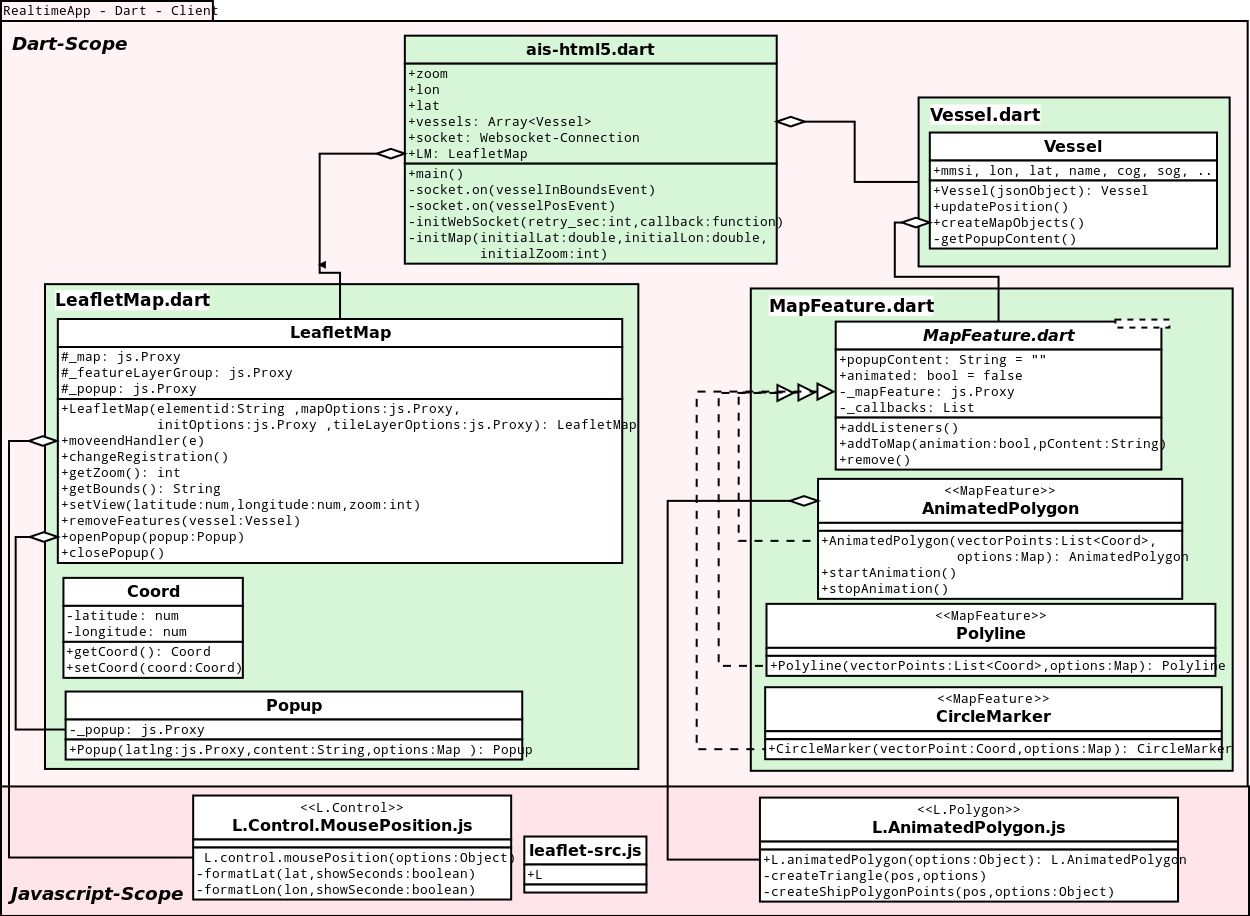
\includegraphics[width=6.2in]{images/Dart-DateienUndKlassen.png}
  \caption[Übersicht Dart-Files]{Schematische Übersicht der Dart-Dateien und -Klassen, sowie der verwendet Javascript-Dateien, siehe auch Anmerkungen zu Abb. \ref{fig:Übersicht Javascript-Files}}
  \label{fig:Übersicht Dart-Files}
\end{figure}


\subsection{HTML5-Client in Google Dart}\label{HTML5-Client in Dart}
Die Implementierung des HTML5-Websocket-Clients in Dart orientiert sich an der Implementierung des HTML5-Websocket-Clients in Javascript. Oberstes Ziel dabei ist es, eine mindestens gleichwertige Funktionalität zu erreichen unter Ausnutzung der sprachspezifischen Vorteile von Google Dart. \\

Die Modularisierung, also die Verteilung der Objekte und Funktionalitäten auf mehrere Dateien, ist in der Dart-Client-Implementierung ähnlich gestaltet wie in Javascript (siehe Abbildungen  \ref{fig:Übersicht Javascript-Files} und \ref{fig:Übersicht Dart-Files}). Die verwendeten Javascript-Dateien (leaflet-src.js, L.AnimatedPolygon.js und L.Control.Mouseposition.js) sind identisch mit denen, die der Javascript-Client (Abschnitt \ref{HTML5-Client in Javascript}) verwendet. Um sie aus Dart heraus nutzen zu können, wird das Dart-Paket js-interop (siehe Abschnitt \ref{js-interop}) eingebunden.
Eine Dart-Anwendung wird über die main-Funktion (in ais-htlml5.dart) gestartet. Die main-Funktion initialisiert den HTML5-Websocket-Client. Im Falle eines erfolgreichen Verbindungsaufbaus mit dem HTML5-Websocket-Server wird die Callback-Funktion ausgeführt, die das LeafletMap-Objekt erstellt. Beide Objekte sind Singletons und bleiben über die Laufzeit der Anwendung erhalten.
Das LeafletMap-Objekt kapselt für die Anwendung den Zugriff auf das Javascript L.Map-Objekt der leaflet.js-Bibliothek (siehe Listing \ref{LeafletMapConstructor}). Dafür wechselt es in den Javascript-Scope der Anwendung und initialisiert in diesem ein L.Map-Objekt und ein L.LayerGroup-Objekt. Beide Objekte werden mit der Anweisung js.retain(...) im Javascript-Scope als globale Variable eingeführt, so dass sie für jede folgende Funktion, die den Javascript-Scope betritt, zur Verfügung stehen.
In der Gegenrichtung muss eine Möglichkeit existieren, vom Javascript-Scope der Anwendung auf den Dart-Code zuzugreifen. Ein Beispiel dafür ist der ‘moveend’-Listener, der Teil der leaflet.js-Bibliothek ist. Für den Javascript-Listener wird ein Dart-Callback.many-Objekt erstellt (moveendHandler(e)), das die changeRegistration-Funktion aus dem Dart-Scope ausführt. Das Callback.many-Objekt in Dart kann im Unterschied zum Callback.once-Objekt mehrmals aufgerufen werden. Das heißt, jedes Mal, wenn im Javascript-Scope der  ‘moveend’-Listener einen  ‘moveend’-Event registriert, ruft er über den Handler die Dart-Funktion changeRegistration() auf. Diese Funktion sendet an den HTML5-Websocket eine Nachricht vom Typ ‘register’ mit den aktuellen Bounds der Karte.

\begin{lstlisting}[caption=Konstruktor des LeafletMap-Objektes mit Zugriff auf den Javascript-Scope, label=LeafletMapConstructor]
LeafletMap(String elementid, js.Proxy mapOptions, js.Proxy initOptions, js.Proxy tileLayerOptions){
    boundsTimeout = initOptions['boundsTimeout']*1000;
    js.scoped(() {
        map = new js.Proxy(js.context.L.Map, elementid, mapOptions);
        featureLayerGroup = new js.Proxy(js.context.L.LayerGroup);
        map.addLayer(featureLayerGroup);
        js.retain(featureLayerGroup);
        var tileLayer = new js.Proxy(js.context.L.TileLayer,tileLayerOptions['tileURL'], tileLayerOptions);
        map.addLayer(tileLayer);
        var mouseOptions = initOptions['mousePosition'];
        if( mouseOptions != false)
        {
          var mousePosition = new js.Proxy(js.context.L.Control.MousePosition, mouseOptions);
          mousePosition.addTo(map);
        }
        map.setView(new js.Proxy(js.context.L.LatLng, initOptions['lat'], initOptions['lon']),initOptions['zoom']);
        js.retain(map);
        map.on('moveend', new js.Callback.many(moveendHandler));
      });
     changeRegistration();
  }
\end{lstlisting}
Der Websocket-Server antwortet auf diese Nachricht mit einer Nachricht vom Typ “VesselsInBoundsEvent” (siehe Listing \ref{websocket-message}).\\
Diese Nachricht und die “VesselPositionEvent”-Nachricht empfängt und verarbeitet der Dart-Client genauso wie der Javascript-Client in Listing \ref{vessel.paintToMap}. Bei der Ausführung der paintToMap-Methode des Vessel-Objektes allerdings besteht ein wichtiger Unterschied darin, dass in Javascript direkt Map-Feature-Objekte der Leaflet.js Bibliothek (L.Polyline, L.AnimatedPolygon und L.CircleMarker) erzeugt werden, wohingegen in Dart der Konstruktor einer Unterklasse (Polyline, AnimatedPolygon oder CircleMarker) von MapFeature aufgerufen wird. Die Konstruktoren aller Unterklassen von MapFeature wechseln in den Javascript-Scope, erstellen dort über einen Proxy ein entsprechendes Objekt aus der Leaflet-Bibliothek und stellen dieses als Attribut des MapFeature-Objektes im Dart-Scope zur Verfügung (siehe Beispiel Klasse Polyline in Listing \ref{Constructor Polyline}).

\begin{lstlisting}[caption= Konstructor des Dart-Objekts Polyline, label = Constructor Polyline]
class Polyline extends MapFeature{
  Polyline(List<Coord> vectorPoints, Map options) {
    js.scoped(() {
      var latlng = js.context.L.LatLng;
      var points =js.array([]);
      for(var x = 0;x < vectorPoints.length; x++)
      {
        var lat =  vectorPoints[x].latitude;
        var lng = vectorPoints[x].longitude;
        points.push(new js.Proxy(latlng,lat,lng ));
      }
      var lineOptions = js.map(options);
      _mapFeature= new js.Proxy(js.context.L.Polyline, points, lineOptions);
      js.retain(_mapFeature);
    });
  }
}
\end{lstlisting}
Auf diese Weise erhält jedes Vessel-Objekt im Array ‘Vessels’, der alle auf der Karte dargestellten Schiffe enthält, als Attribut .feature und/oder .polygon eine Assoziation zu einer Dart-Klasse, die über einen js.Proxy die Verwaltung des dazugehörigen Javascript-Objektes im DOM-Baum für die Anwendung kapselt.

Nach demselben Prinzip funktionieren Popups in der Anwendung.

Um Popups auf den MapFeature-Objekten über MouseEvents öffnen und schließen zu können, werden auf den mouseover und den mouseout-EventListener des Javascript-Proxies eines jeden MapFeature-Objektes EventHandler als Dart-Callback.many-Funktionen registriert (siehe Listing \ref{EventHandling}). Diese Callback.many-Funktionen führen im Dart-Scope alle notwendigen Anweisungen aus. Zum Beispiel erstellt der MouseoverHandler ein Dart-Popup-Objekt, das im Konstruktor einen Proxy zu einem L.Popup-Objekt erstellt und als Instanzvariable speichert. Operationen auf dem L.Map-Objekt müssen über das Dart LeafletMap-Objekt ausgeführt werden, das den Javascript-Proxy zum L.Map-Objekt verwaltet. Im Falle des onMouseoverHandlers, wird das Dart-Popup-Objekt der Funktion LMap.openPopup(popup) übergeben, die Funktion wechselt in den Javascript-Scope und öffnet auf dem L.Map-Objekt den Javascript-Proxy des Popup-Objektes (siehe Listing \ref{LeafletMap-Objekt})
\\
\begin{lstlisting}[caption=EventHandling mithilfe von Callback-Funktionen, label= EventHandling]
void addListeners(){
    onMouseoutHandler(e){
      LMap.closePopup();
    }
    onMouseoverHandler(e){
      var ll = e.latlng;
      ll =  new js.Proxy(js.context.L.LatLng ,ll.lat, ll.lng);
      var popupOptions = {'closeButton': false,
                        'autoPan': false,
                        'maxWidth': 150, 
                        'offset' : [50,-50]};
      var popup = new Popup(ll, popupContent, popupOptions);
      LMap.closePopup();
      LMap.openPopup(popup);
    }
    
    _callbacks.add(new js.Callback.many(onMouseoverHandler));
    _callbacks.add(new js.Callback.many(onMouseoutHandler));
    
    _mapFeature.on('mouseover', _callbacks[0]);
    _mapFeature.on('mouseout', _callbacks[1]);
  }
  \end{lstlisting}
  \begin{lstlisting}[caption=Zugriff auf das L.Map-Objekt (im Javascript-Scope) über das LeafletMap-Objekt (im Dart-Scope) in LeafletMap.dart, label= LeafletMap-Objekt]
class LeafletMap {
  js.Proxy map;
  ...
  closePopup(){
    js.scoped((){
      map.closePopup();
    });
  }

  openPopup(Popup popup){
    js.scoped((){
      map.openPopup(popup._popup);
    });
  }
...
}  
  \end{lstlisting}